%%%% Catálogo de reglas de negocio %%%%

\section{Modelos de ciclo de vida}

	%Descripción de ciclo de vida
	\hypertarget{CV:CuentaSolicitante}{}
	\subsection{Ciclo de vida de una orden}

		Una orden puede encontrarse en uno o varios estados que definen su ciclo de vida en el sistema, donde cada estado define las acciones que puede o no realizar el \hyperlink{A:Cliente}{Cliente}. Los estados y transiciones posibles para una orden se muestran en la figura \ref{fig:CV:Orden}.
	
		A continuación se describe cada estado.

		%Descripción de estados
		\begin{itemize}

			\item \hypertarget{cv:cs:edo:Nueva}{\textit{Nueva}}. Estado con el que inicia una orden. Es necesario que el cliente haya seleccionado una de las opciones disponibles para agregarla al carrito de compras, a este estado se llega mediante el \hyperlink{CU1}{CU1 Seleccionar Pizza}. A partir de este estado se puede pasar solamente a los estados de \textbf{En preparación} y \textbf{Cancelada}.

			\item \hypertarget{cv:cs:edo:EnPreparación}{\textit{En preparación}}. La orden pasa a este estado cuando el cliente decide no seguir agregando elementos a su carrito de compras, a este estado se llega mediante el \hyperlink{CU3}{CU3 Realizar la Compra}.A partir de este estado se puede pasar solamente a los estados de \textbf{Terminada} y \textbf{Cancelada}.
			
			\item \hypertarget{cv:cs:edo:Terminada}{\textit{Terminada}}.  La orden pasa a este estado cuando el cliente decide seguir agregando elementos a su carrito de compras,a este estado se llega mediante el \hyperlink{CU1}{CU1 Seleccionar Pizza}.A partir de este estado se puede pasar solamente a los estados de \textbf{Enviada} y \textbf{Cancelada}.
			
			\item \hypertarget{cv:cs:edo:Enviada}{\textit{Enviada}}.  La orden pasa a este estado cuando el cliente ingresa sus datos y su método de pago al sistema, a este estado se llega mediante los  \hyperlink{CU4}{CU4 Confirmar Datos de Compra} y \hyperlink{CU5}{CU5 Seleccionar Método de Pago}.A partir de este estado se puede pasar solamente a los estados de \textbf{Entregada} y \textbf{Cancelada}.
			
			\item \hypertarget{cv:cs:edo:Entregada}{\textit{Entregada}}.  Estado con el que finaliza la orden.La orden pasa a este estado cuando el sistema registró la compra que el cliente realizó junto con sus datos y su método de pago para que el cliente pueda descargar su comprobante de compra, a este estado se llega mediante los  \hyperlink{CU4}{CU4 Confirmar Datos de Compra} y \hyperlink{CU5}{CU5 Seleccionar Método de Pago}.Ya no existen más transiciones a partir de este estado.
			
			\item \hypertarget{cv:cs:edo:Cancelada}{\textit{Cancelada}}.  Estado con el que finaliza la orden. La orden pasa a este estado cuando el cliente elimina todos los elementos que se encuentran agregados en su carrito de compras, a este estado se llega mediante el \hyperlink{CU2}{CU2 Ver Carrito de Compras}.Ya no existen más transiciones a partir de este estado.
		\end{itemize}

		%Maquina de estados
\begin{figure}[h]
	
	\begin{center}				
		
		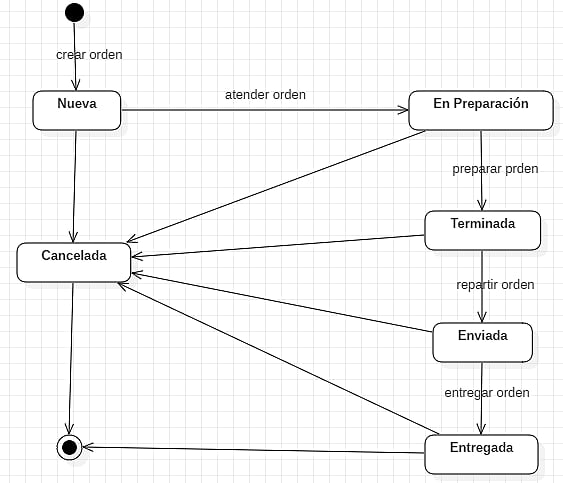
\includegraphics[scale=0.50]{imagenes/CiclosDeVida/cv-Orden.png}
		\caption{Ciclo de vida de una cuenta de solicitante}
		\label{fig:CV:Orden}
		
	\end{center}
	
\end{figure}
		\noindent Rererenciada por: 
		
			\begin{itemize}

				\item \textit{Actores:} \hyperlink{A:Cliente}{Cliente}

				\item \textit{Casos de uso:} \hyperlink{CU1}{CU1 Seleccionar Pizza}, \hyperlink{CU2}{CU2 Ver Carrito de Compras}, \hyperlink{CU3}{CU3 Realizar la Compra},\hyperlink{CU4}{CU4 Confirmar Datos de Compra} y \hyperlink{CU5}{CU5 Seleccionar Método de Pago}

			\end{itemize}

